\begin{XeClass}{LocalDirAllocator}
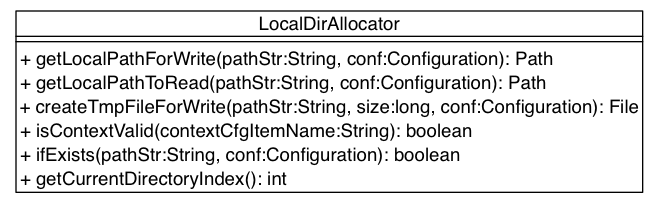
\includegraphics[width=\textwidth]{cdig/LocalDirAllocator.png}
     
 该类是创建文件时磁盘分配round-robin模式的一种实现。
 它实现的方式就是持续跟踪磁盘最后是被一个文件写在什么位置的。

    \begin{XeMethod}{\XePublic}{Path}{getLocalPathForWrite}
         
 为了写入获得本地文件系统的一个路径

    \end{XeMethod}

    \begin{XeMethod}{\XePublic}{Path}{getLocalPathToRead}
         
 为了读入获得本地文件系统的一个路径

    \end{XeMethod}

    \begin{XeMethod}{\XePublic}{File}{createTmpFileForWrite}
         
 为了写入创建一个临时文件

    \end{XeMethod}

    \begin{XeMethod}{\XePublic}{boolean}{isContextValid}
         
 判断内容是否有效

    \end{XeMethod}

    \begin{XeMethod}{\XePublic}{boolean}{ifExists}
         
 判断路径是否存在

    \end{XeMethod}

    \begin{XeMethod}{}{int}{getCurrentDirectoryIndex}
         
 获得当前目录的索引号

    \end{XeMethod}

    \begin{XeInnerClass}{AllocatorPerContext}
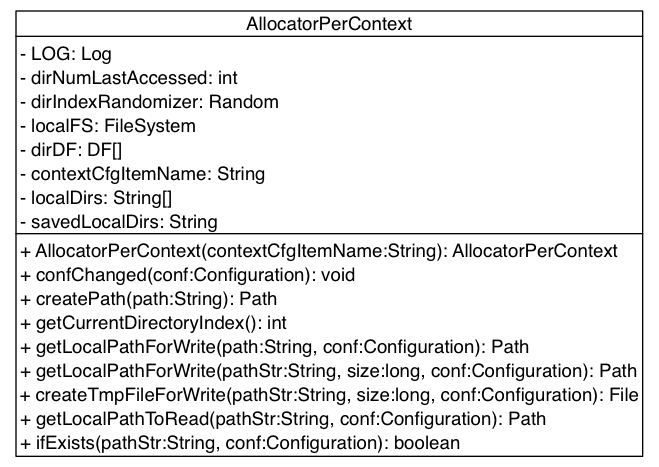
\includegraphics[width=\textwidth]{cdig/AllocatorPerContext.png}
        
        \begin{XeMethod}{\XePrivate}{void}{confChanged}
             
 改变配置信息

        \end{XeMethod}

        \begin{XeMethod}{\XePrivate}{Path}{createPath}
             
 创建路径

        \end{XeMethod}

        \begin{XeMethod}{\XePublic \\ \XeSync}{Path}{getLocalPathForWrite}
             
 采用round-robin模式从本地文件系统中获取一个路径

        \end{XeMethod}

        \begin{XeMethod}{\XePublic}{File}{createTmpFileForWrite}
             
 创建一个可供写入的临时文件

        \end{XeMethod}

        \begin{XeMethod}{\XePublic \\ \XeSync}{Path}{getLocalPathToRead}
             
 搜索所有的配置目录,返回一个找到的完全路径

        \end{XeMethod}

        \begin{XeMethod}{\XePublic \\ \XeSync}{boolean}{ifExists}
             
 搜索所有的配置目录看所要找的文件是否存在。

        \end{XeMethod}

    \end{XeInnerClass}
\end{XeClass}
